\documentclass{beamer}
\usetheme{}
\usecolortheme{dolphin}           
\useinnertheme{circles}
\setbeamertemplate{itemize items}[default]
\setbeamertemplate{enumerate items}[default]
\usepackage[T1]{fontenc}
\usepackage[utf8]{inputenc}
\usepackage{lmodern}
\usepackage{amsmath}
\usepackage{booktabs} 
\usepackage{graphicx}        
\usepackage{array}
\usepackage{color}
\usepackage{svg}
\makeatletter
\def\zapcolorreset{\let\reset@color\relax\ignorespaces}
\def\colorrows#1{\noalign{\aftergroup\zapcolorreset#1}\ignorespaces}
\makeatother
\graphicspath{{/home/swl/Dropbox/ucd/advanced_macro/figures/}} 
\setbeamertemplate{navigation symbols}{}
%--------------------------------------
%%%% DETAILS TITLE PAGE %%%%
%--------------------------------------
\title{Identification in macroeconomics}
\author{School of Economics, University College Dublin}
\date{Spring 2018}
\begin{document}

%--------------------------------------
\begin{frame}
 \titlepage
\end{frame}
%--------------------------------------

%--------------------------------------
\begin{frame}
  Some important questions in macroeconomics include
  \begin{itemize}
     \item Why do some countries grow faster than others?
     \medskip
     \item What causes business cycle fluctuations?
     \item How does monetary or fiscal policy affect the economy?
   \end{itemize} 
\end{frame}
%--------------------------------------

%--------------------------------------
\begin{frame}
  The answers to these questions are often 
  \begin{enumerate}
    \item Unknown
    \item Difficult to answer
  \end{enumerate}
  \medskip
  A major complication - as in any empirical field - is identification.
\end{frame}
%--------------------------------------

%--------------------------------------
\begin{frame}
  What is identification?
  \begin{itemize}
    \item Necessary condition for the existence of consistent estimators
    \item i.e. when sample size increases, the estimator will converge, probabilistically, to parameters unknown value
  \end{itemize}
  \medskip
  Analytically, identification entails whether or not the unknown parameter value can be deduced from the observed data
  \begin{itemize}
    \item Consistent estimators may exist under number of assumptions, i.e. central limit theorem etc.
  \end{itemize}
\end{frame}
%--------------------------------------

%--------------------------------------
\begin{frame}
 For a general definition of identification, let $P$ be the true distribution of observed data $X$ which can be modeled by
 \begin{align}
   \mathbf{P} = \{P_{\theta}: \theta \in \Theta  \}
 \end{align}
 Assuming that 
 \begin{align}
   P \in \mathbf{P}
 \end{align}
 or that there is a correctly specified model with parameters $\theta \in \Theta$ such that $P \in \mathbf{P}$.
 Of course we are interested in $\theta$  
\end{frame}
%--------------------------------------

%--------------------------------------
\begin{frame}
  Suppose that we know for a fact that $P \in \mathbf{P}$ which entails that $\theta \in \Theta$ for $P_{\theta} \in \mathbf{P}$
  \begin{itemize}
    \item Only problem is that we can't distinguish between $\theta \in \Theta$ from $\theta^* \in \Theta$
  \end{itemize}
  \medskip
  So from our knowledge about $P$ alone we can only say that 
  \begin{align}
    \theta \in \Theta_0(P)= \{\theta \in \Theta: P_{\theta} = P\}
  \end{align}  
\end{frame}
%--------------------------------------

%--------------------------------------
\begin{frame}
  $\Theta_0(P)$ is the identified set
  \begin{itemize}
    \item $\theta$ is identified if $\Theta_0 (P)$ is a singleton for all $P \in \mathbf{P}$
  \end{itemize} 
  \medskip
  $\mathbf{P}$ should be interpreted as a structural model for the distribution of observed data $X$
\end{frame}
%--------------------------------------

%--------------------------------------
\begin{frame}
  Why should we care about a structural model? As we can calculate interesting statistics from $P$
  \begin{itemize}
    \item Predictors, conditional probabilities, etc.    
  \end{itemize}
  \medskip
  These statistics can provide useful insights about the data but not the mechanisms that generate the data.
  In the identified model the structure of the data $\mathbf{P}$ is given by unknown value $\theta \in \Theta$.
  \begin{itemize}
    \item A central question is what we can learn from $\theta$, under certain conditions, from observed distribution $P$
  \end{itemize}
\end{frame}
%--------------------------------------

%--------------------------------------
\begin{frame}
  Let's consider a more practical example looking at the FED interest rates:
  In 2008 the FED lowered the rates in a reaction to the crisis.
  \begin{itemize}
    \item Lowering interest rates should encourage spending; stimulate economic activity
  \end{itemize}
  \medskip
  Changes in interest rate are a source of variation in monetary policy which can be used in the model. 
\end{frame}
%--------------------------------------

%--------------------------------------
\begin{frame}
  \begin{figure}
    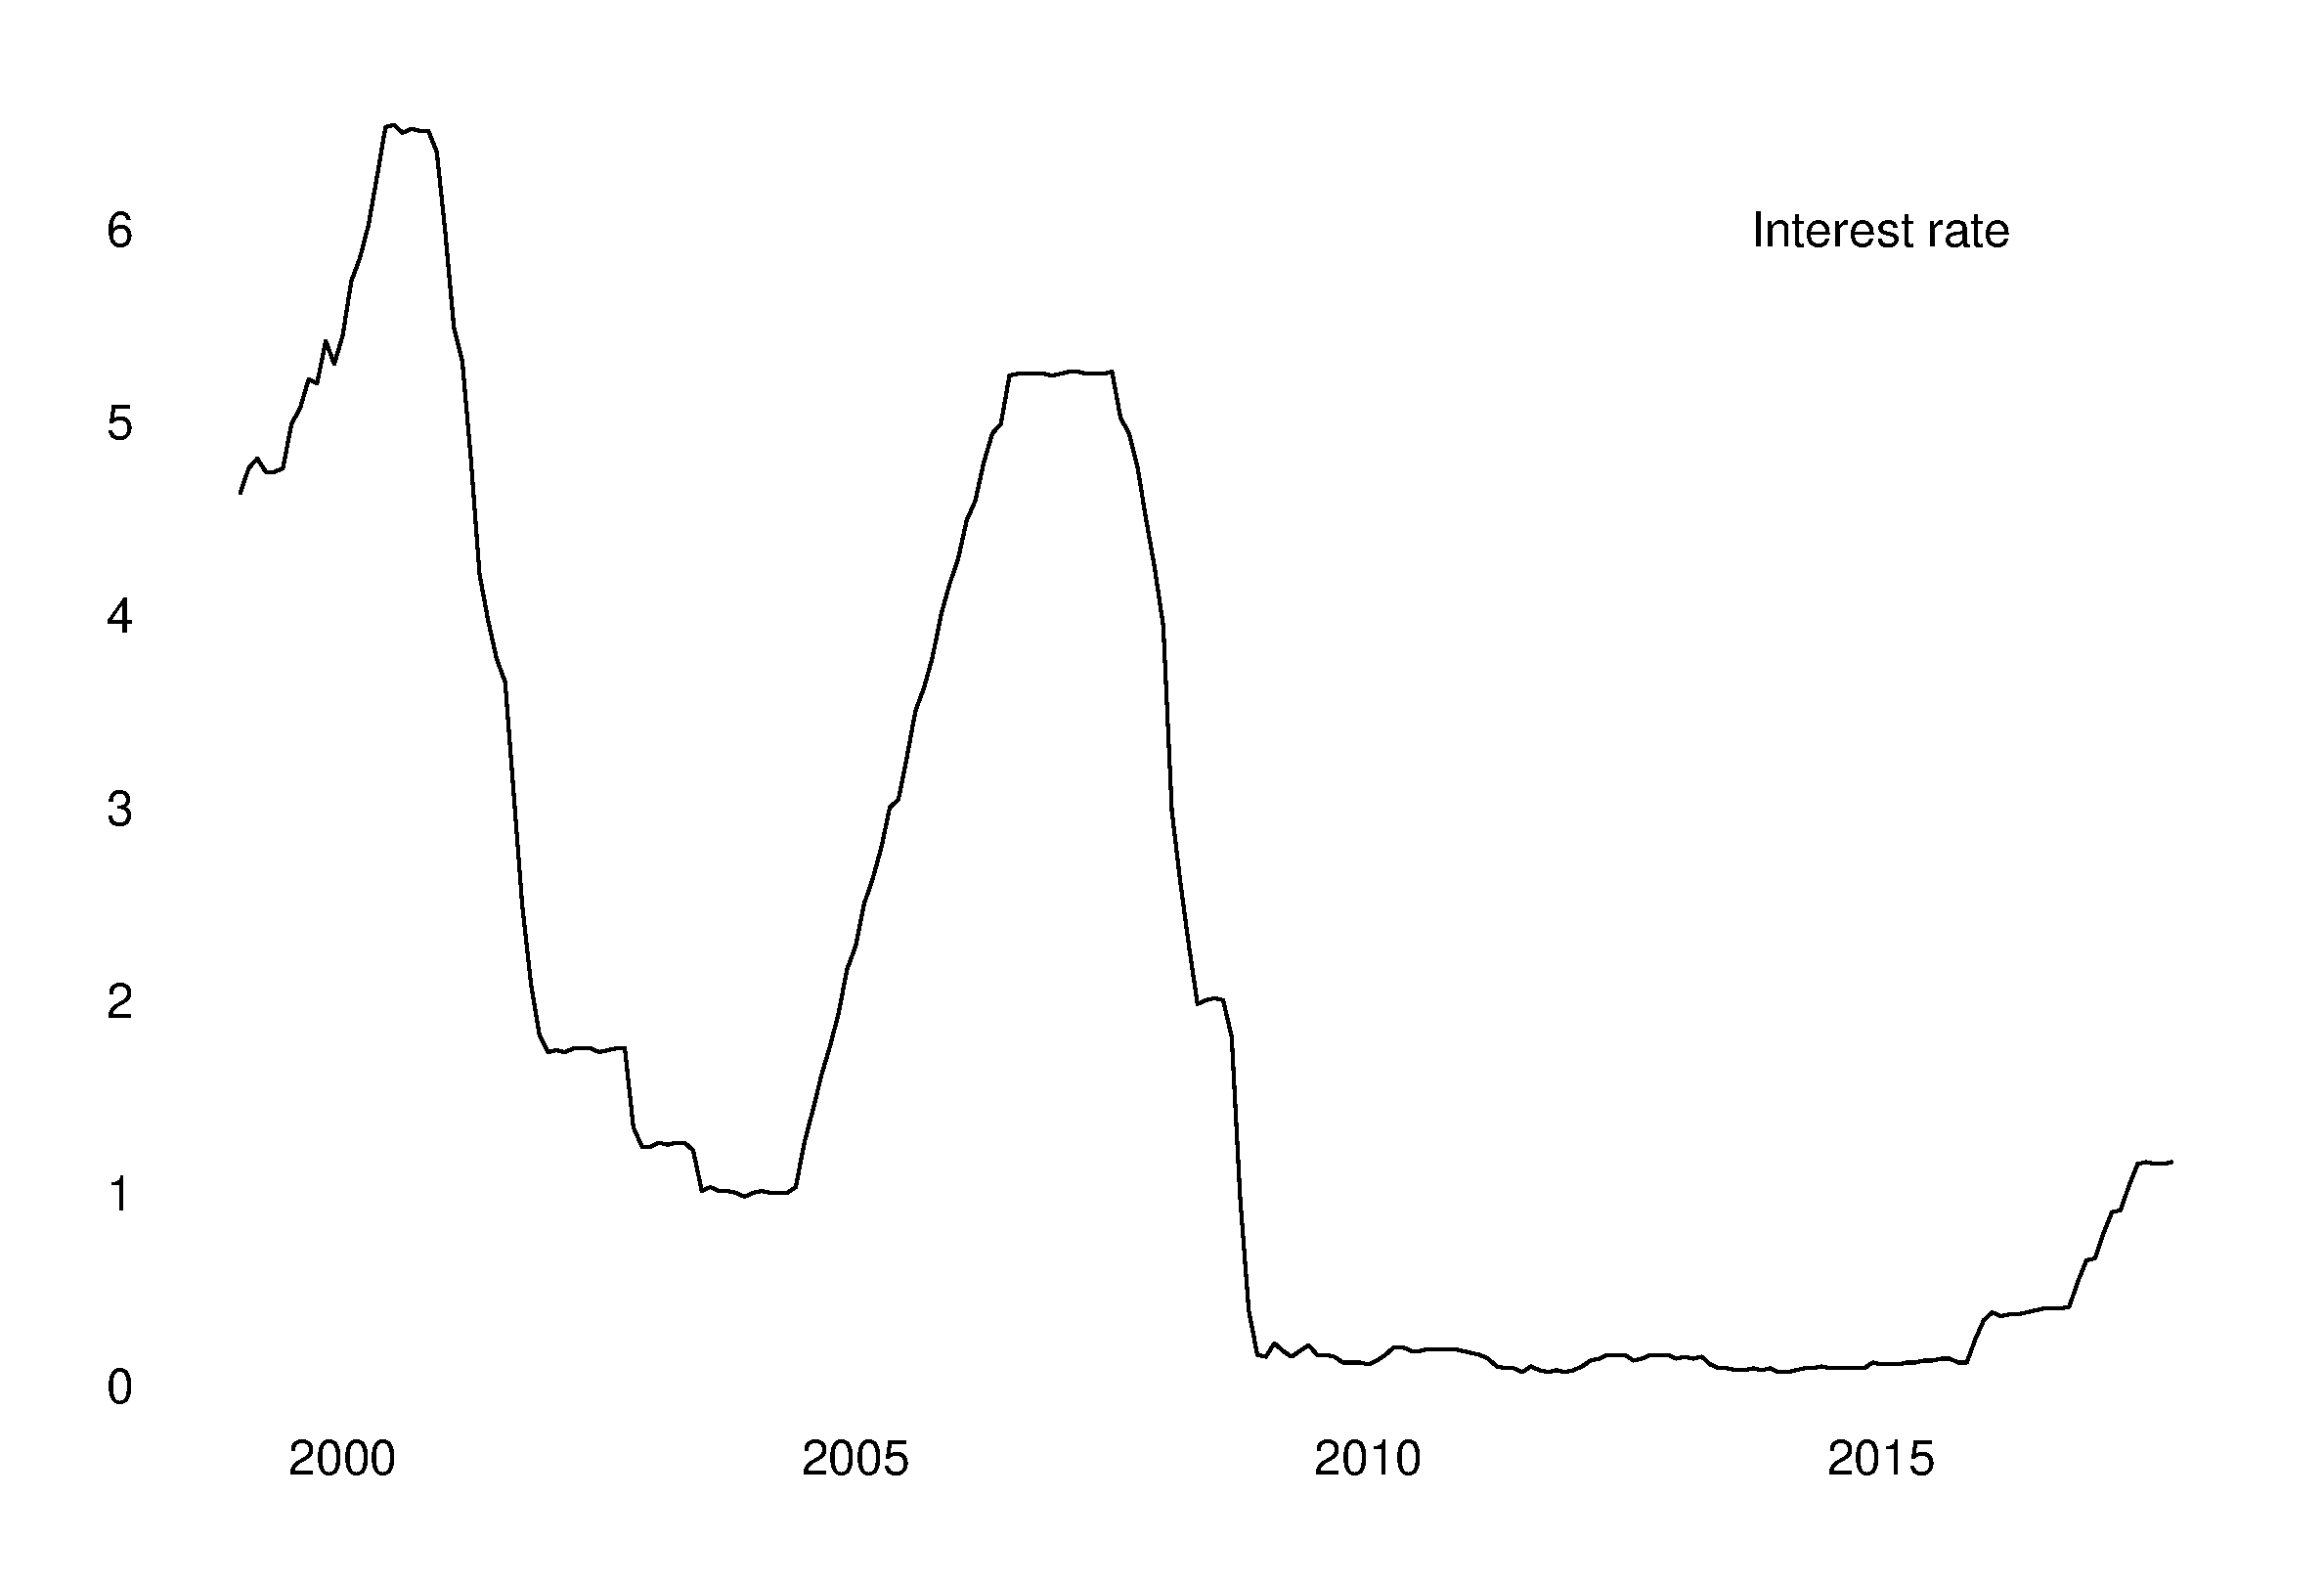
\includegraphics[scale=.3]{effective_rate.eps}
  \end{figure}
\end{frame}
%--------------------------------------

%--------------------------------------
\begin{frame}
 Can estimate effect of interest rate on economic output using following model: 
  \begin{align*}
    \Delta GDP_t = \alpha + \beta \Delta i_t + \epsilon_t
  \end{align*}
  \medskip
  Fit model to data using OLS; possible estimate $\beta > 0$
\end{frame}
%--------------------------------------


%--------------------------------------
\begin{frame}
  Simple OLS regression would lead to conclusion that reduction in interest rate correlates/causes decreases in output
  \begin{itemize}
    \item Lowering interest rate harms the economy
  \end{itemize}
  \medskip
  Policy implication would be to increase interest rates to stimulate economic activity.
  \begin{itemize}
    \item Sticking to evidence-based policy
  \end{itemize}
\end{frame}
%--------------------------------------

%--------------------------------------
\begin{frame}
  FED does not change interest rates randomly, but change due to some factors affecting the economy
  \begin{itemize}
    \item Interest rates are endogenous    
    \item Around 2008 think falling house prices and their effect on bank balance sheets
  \end{itemize}
    \medskip
  These other factors confound effect of change in monetary policy
  \begin{itemize}
    \item i.e. OLS regression does not capture isolated effect of interest rate
  \end{itemize}
\end{frame}
%--------------------------------------

%--------------------------------------
\begin{frame}
  Paramount in macroeconomic research is the role of dynamics, and there are two important challenges:
  \begin{enumerate}
    \item Difficult to identify exogenous variation in macroeconomic policy
    \item Natural experiment that can be identified are rarely those required to answer questions we're interested in. 
  \end{enumerate}
  \medskip
  As a result, there is an external validity problem.
\end{frame}
%--------------------------------------


%--------------------------------------
\begin{frame}
 There are some additional important issues : 
 \begin{enumerate}
   \item Dynamic nature of monetary and fiscal policy make it high dimensional; can have effect on both short and long run
   \item Effects of fiscal shocks depends on monetary policy (constrained by zero lower bound) and tax policy response
   \item Effect of policy depends on the economy
   \item Degree to which a policy is a surprise affects when and how strongly an economy reacts  
 \end{enumerate}
 \medskip
 This entails that macroeconomic research tends to be structural in nature
 \begin{itemize}
   \item Different from other empirical economic research which seeks to identify causal effects
 \end{itemize} 
\end{frame}
%--------------------------------------

%--------------------------------------
\begin{frame}
  As in any quantitative field macroeconomics relies on the use of statistical methods and thus on the use of moments
  \begin{itemize}
    \item Moments characterises the statistical distribution and are most commonly taken around the mean
  \end{itemize}
  \medskip
  In terms of econometrics we can distinguish between identified and unidentified moments
  \begin{enumerate}
    \item Unidentified: Simple statistics such as means, variances, and correlations
    \item Identified: Statistics derived from empirical strategies or causal effect estimates 
  \end{enumerate}
\end{frame}
%--------------------------------------

%--------------------------------------
\begin{frame}
 Identified moments are designed to help uncover causal effects (micro) or responses to structural shocks (macro).
 \begin{enumerate}
   \item Micro moments are constructed using microeconomic data on behaviour of individuals and firms
   \item Macro moments use aggregated data to identify equilibrium outcomes; informative about what type of world we live in 
  \end{enumerate} 
\end{frame}
%--------------------------------------

%--------------------------------------
\begin{frame}
  Do identified moments correspond to structural parameters?
  \begin{itemize}
    \item They do in some cases: Labour supply elasticity in labour economics
  \end{itemize}
  \medskip
  In other cases they don't
  \begin{enumerate}
    \item Marginal propensity to consume following transitory fiscal rebate
    \item Estimate of regional fiscal multiplier
  \end{enumerate}
  \medskip
  In cases where they don't correspond you need a theoretical framework to go from the identified moments to the macroeconomic question of interest.
\end{frame}
%--------------------------------------

%--------------------------------------
\begin{frame}
 Finally there is the issue of data and the unit-of-analysis which means that identification can be done at
  \begin{enumerate}
    \item Aggregate level; focusing on single country
    \item Cross-sectional level; e.g. across countries or within country
  \end{enumerate}
  \medskip
  Cross-sectional identification is a fairly recent development
  \begin{itemize}
    \item Due to improvements in data collection
    \item Cross-sectional identification brings additional estimation challenges
  \end{itemize}
\end{frame}
%--------------------------------------

%--------------------------------------
\begin{frame}
 Majority of studies are based on U.S. economy
 \begin{itemize}
   \item Largest economy in the world
   \item Technological leader
   \item Best data availability
 \end{itemize}
\end{frame}
%--------------------------------------

%--------------------------------------
\begin{frame}
  Example of aggregate identification for fiscal stimulus
  \begin{enumerate}
    \item Evidence coming from wars
    \item Evidence coming from VARs
  \end{enumerate}
  \medskip
  NB - We will discuss VARs in more detail than you could wish for - or desire - later during the course.
\end{frame}
%--------------------------------------

%--------------------------------------
\begin{frame}
  \begin{figure}
    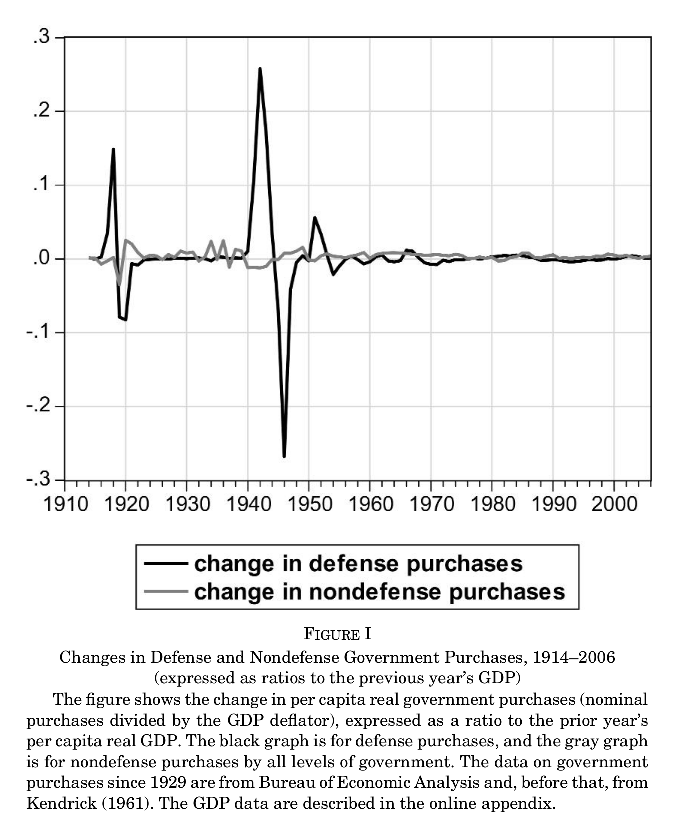
\includegraphics[scale=.5]{barro_redlick1.eps}
  \end{figure}
  Barro \& Redlick, 2011
\end{frame}
%--------------------------------------

%--------------------------------------
\begin{frame}
  \begin{figure}
    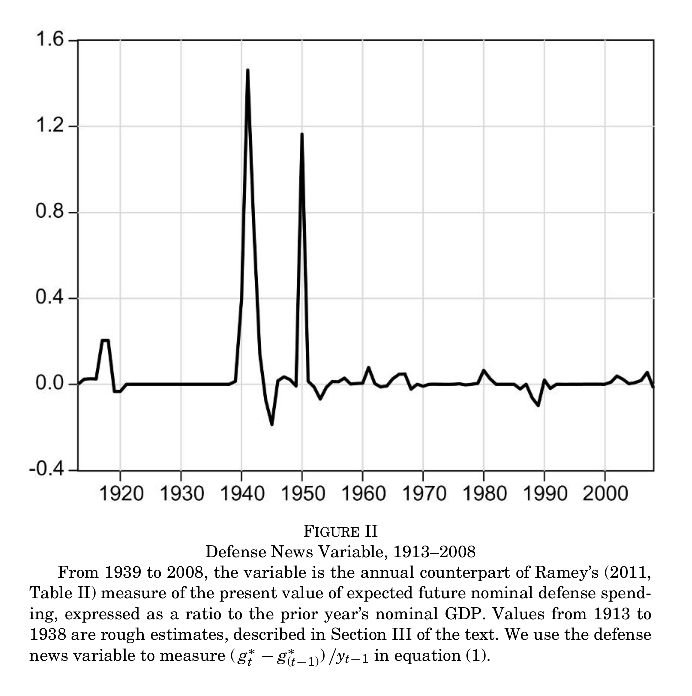
\includegraphics[scale=.5]{barro_redlick2.eps}
  \end{figure}
  Barro \& Redlick, 2011
\end{frame}
%--------------------------------------

%--------------------------------------
\begin{frame}
  \begin{figure}
    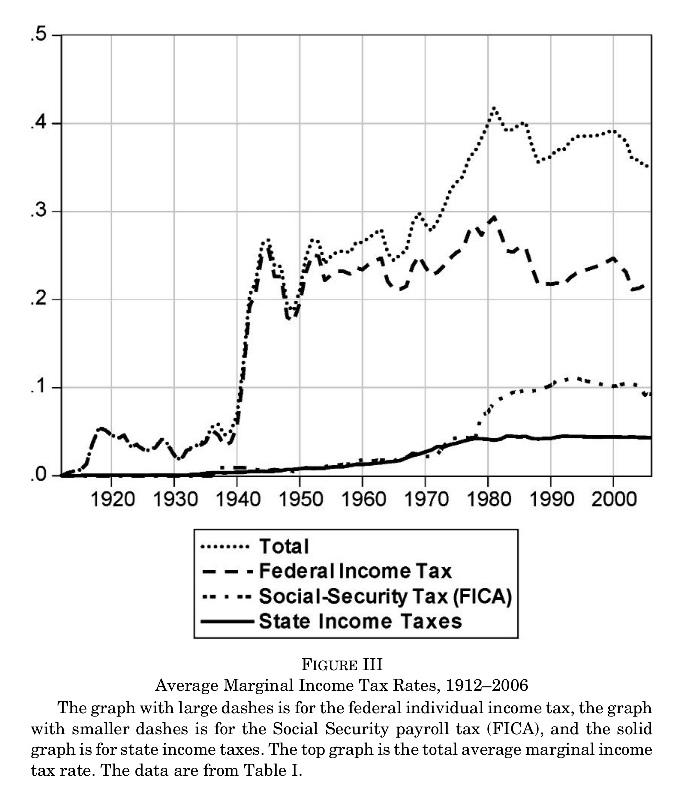
\includegraphics[scale=.5]{barro_redlick3.eps}
  \end{figure}
  Barro \& Redlick, 2011
\end{frame}
%--------------------------------------

%--------------------------------------
\begin{frame}
  \begin{figure}
    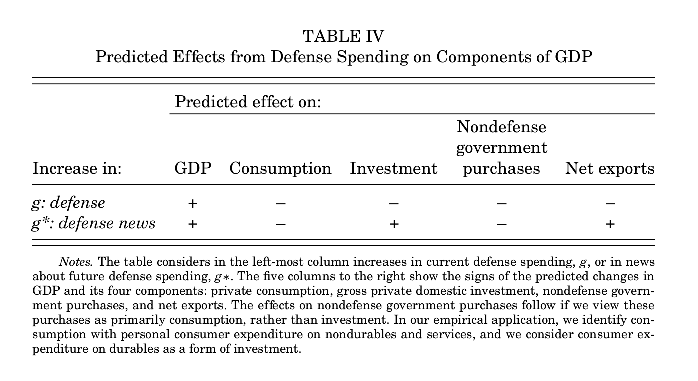
\includegraphics[scale=.5]{barro_redlick4.eps}
  \end{figure}
  Barro \& Redlick, 2011
\end{frame}
%--------------------------------------

%--------------------------------------
\begin{frame}
 Let's turn the attention to evidence for the non-neutrality of monetary policy. 
 Nakamura \& Steinsson highlight three prominent pieces of evidence
 \begin{enumerate}
   \item Bad policy by the FED prior to the Great Depression which made things worse
   \item The Volcker disflation
   \item Break in volatility of US real exchange rate
 \end{enumerate} 
\end{frame}
%--------------------------------------

%--------------------------------------
\begin{frame}
  Provided evidence gives a glimpse into preferred empirical methods
  \begin{itemize}
    \item Two cases are exclusively based on historical events
    \item One is example of identification based on discontinuity
  \end{itemize}
  \medskip
  Not appearing in this list: VARs
\end{frame}
%--------------------------------------

%--------------------------------------
\begin{frame}
  Four prevalent approaches
  \begin{enumerate}
    \item Large shocks
    \item Narrative record to identify shocks
    \item Discontinuity-based identification    
    \item 'Controlling' for confounding factors, i.e. VAR methods
  \end{enumerate}
\end{frame}
%--------------------------------------

%--------------------------------------
\begin{frame}
  Gold standard of empirical science is the controlled experiment
  \begin{itemize}
    \item Hard to implement when one is interested in the effect of monetary policy
  \end{itemize}
  \medskip
  Need to look for 'natural experiments' or large shocks
  \begin{itemize}
    \item i.e. situations where policy changes are relatively large to potential confounding factors that cannot be accounted for
    \item These type of changes are few and far between
  \end{itemize}
\end{frame}
%--------------------------------------

%--------------------------------------
\begin{frame}
  Friedman \& Schwartz argue that three policy actions taken by the FED in the interbellum were
  \begin{enumerate}
    \item 'of major magnitude'
    \item 'cannot be regarded as necessary or inevitable economic consequences of contemporary changes in money income and prices'
  \end{enumerate}
  \medskip
  They also argue that '\textit{the results are so consistent and sharp as to leave little doubt about their interpretation.}'
  The dates of the events are
  \begin{enumerate}
    \item January-June 1920
    \item October 1931
    \item July 1936 - January 1937
  \end{enumerate}
\end{frame}
%--------------------------------------

%--------------------------------------
\begin{frame}
  \begin{figure}
    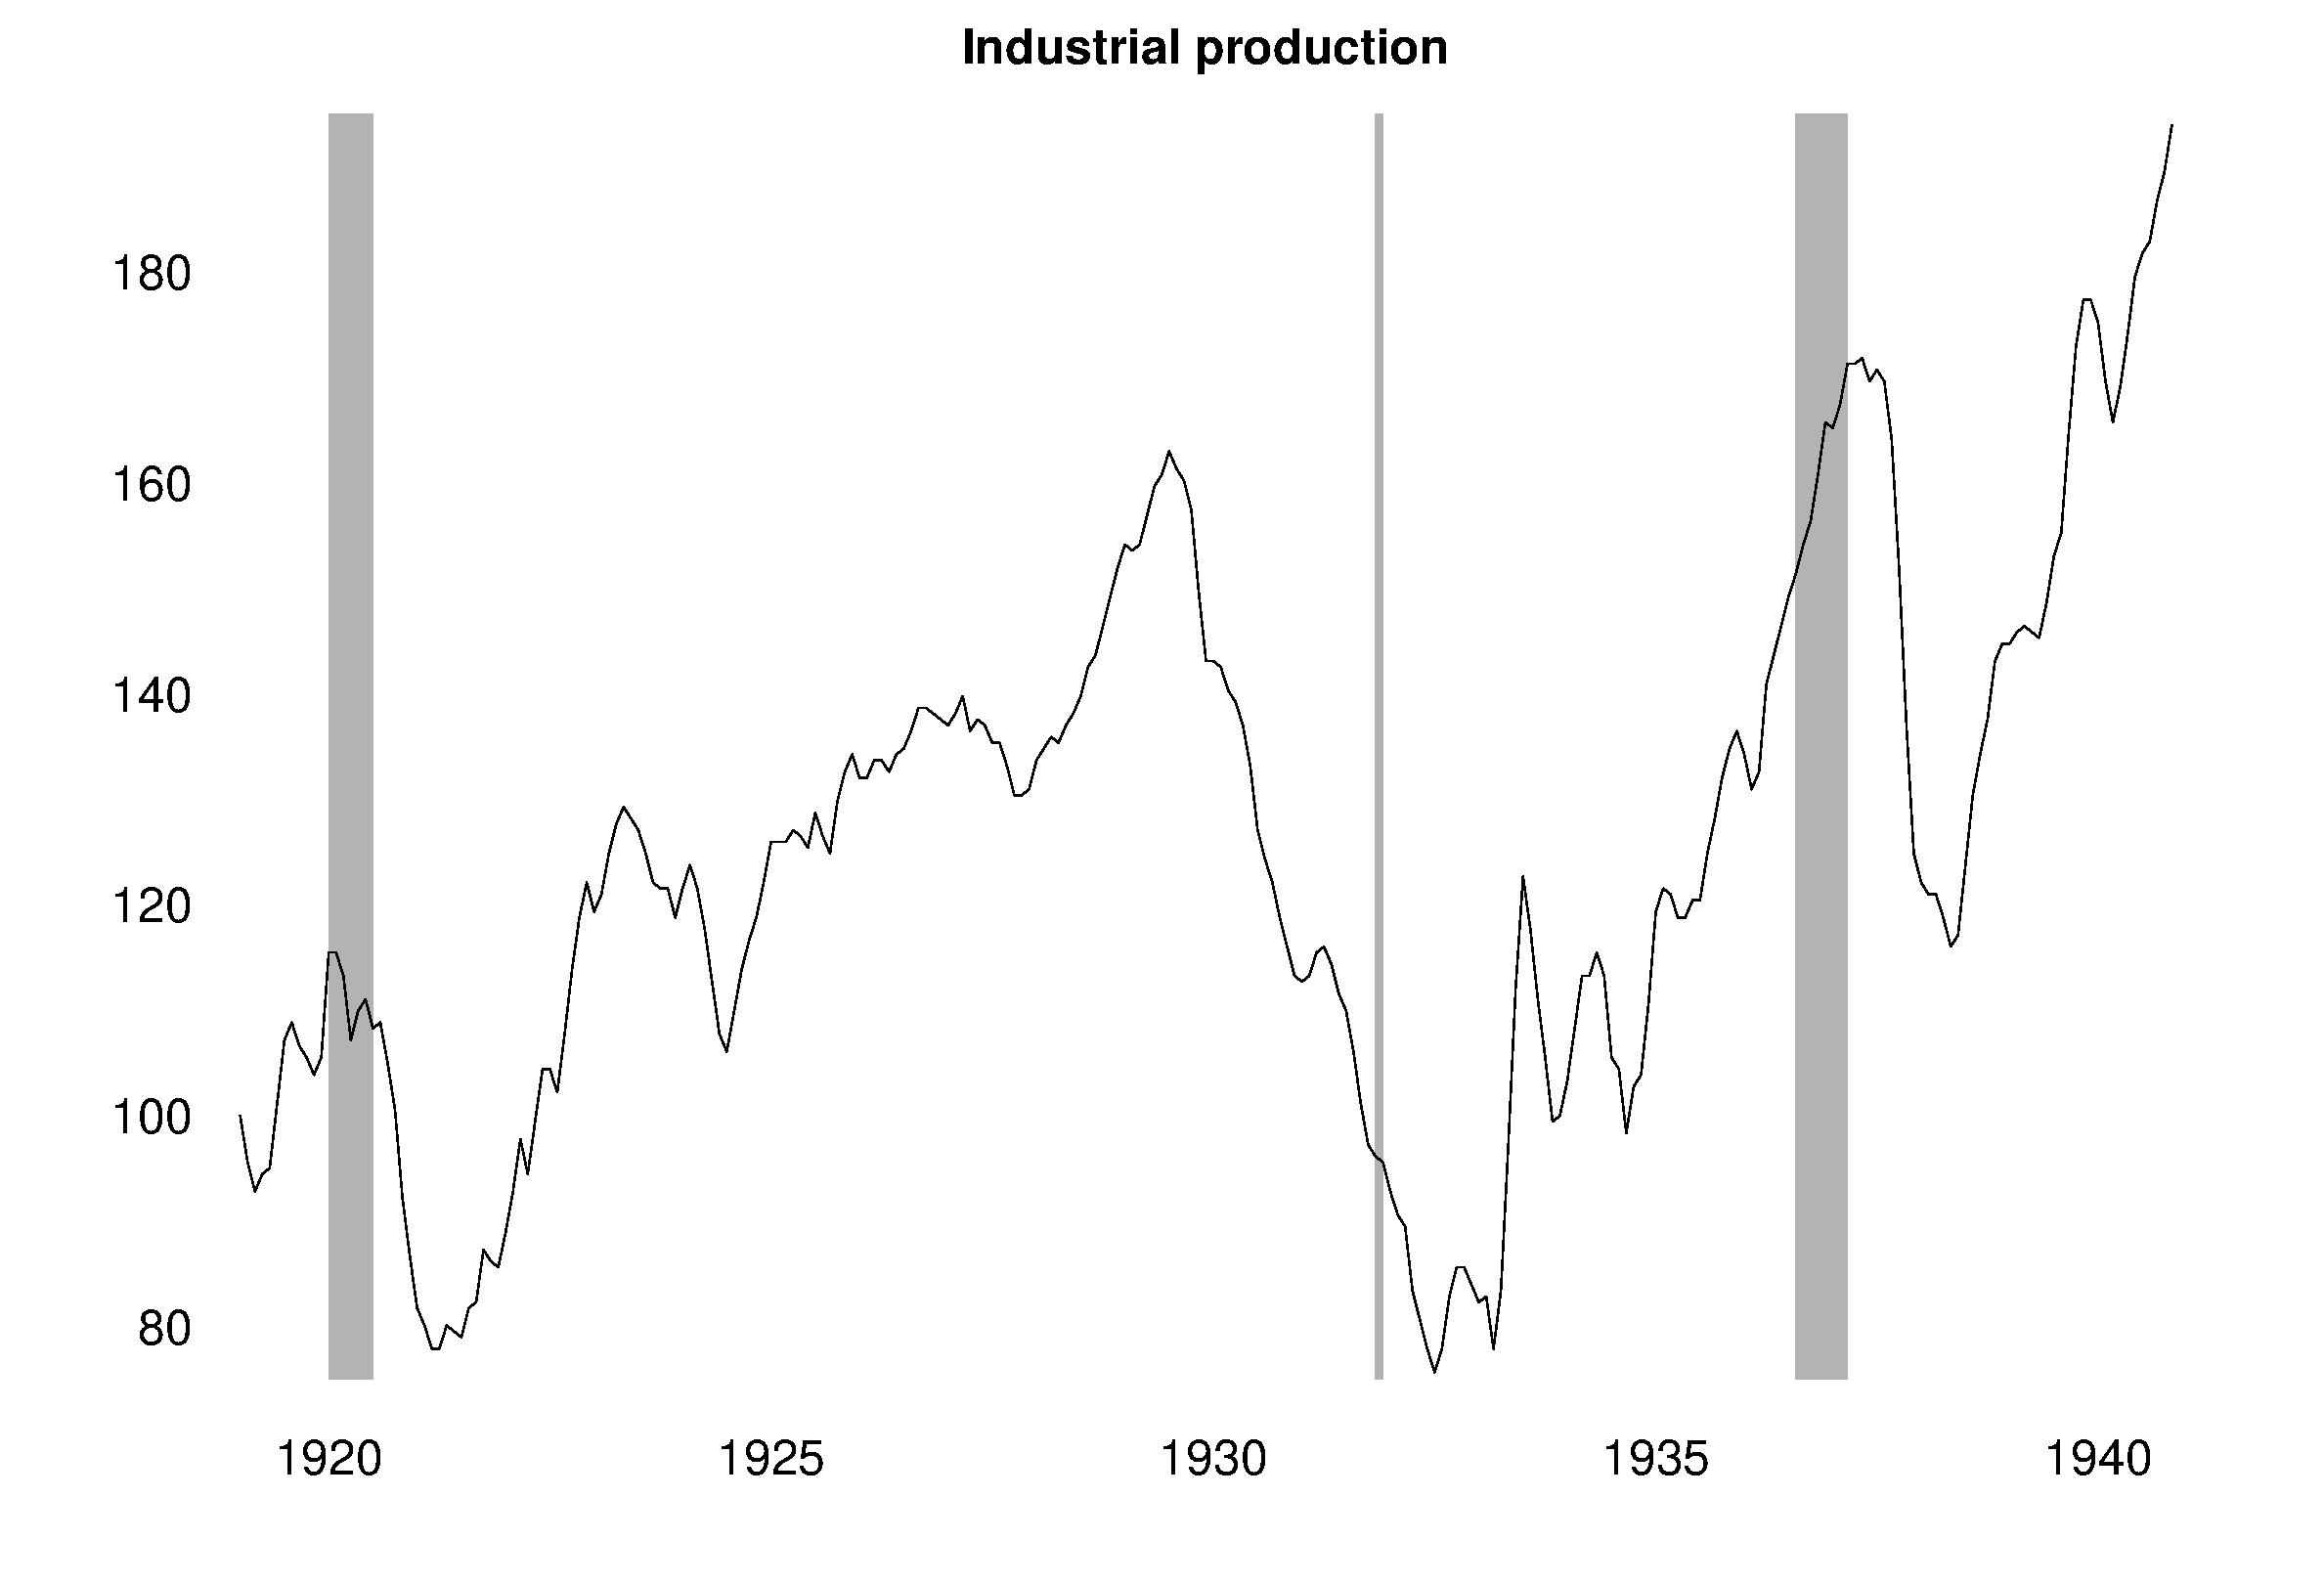
\includegraphics[scale=.3]{industrial_production.eps}
  \end{figure}
\end{frame}
%--------------------------------------

%--------------------------------------
\begin{frame}
  What where these policy mistakes Friedman \& Schwartz identified?
  Let's look at the decision made in October 1931
  \begin{itemize}
    \item FED raised the discount rate from 1.5\% to 3.5\%
    \item Response to speculative attack on US dollar following Britain leaving the gold standard
  \end{itemize}
  \medskip
  FED tightened policy at a time that industrial production was decreasing rapidly; this might seem like clear monetary shock.
  \begin{itemize}
    \item Subsequent fall in industrial production not much different from preceding period
    \item Unclear how much of decrease can be attributed to policy shock
  \end{itemize}
\end{frame}
%--------------------------------------

%--------------------------------------
\begin{frame}
 Volcker  disflation followed after Volcker was appointed as chairman of the Federal Reserve Board in August 1979
 \begin{itemize}
   \item After end of Korean War in 1953 inflation was stable and low, but started to rise in late 1960s
   \item During 1970s inflation was high and volatile, often in double digits
 \end{itemize}
 \medskip
 Monetary policy was characterised by 'stop-go'
 \begin{itemize}
   \item Tight when the public was concerned about inflation, loose when public was concerned about unemployment
 \end{itemize}
  In November 1980 Volcker broke with this modus operandi and targeted deliberate disinflation  
\end{frame}
%--------------------------------------

%--------------------------------------
\begin{frame}
  \begin{figure}
    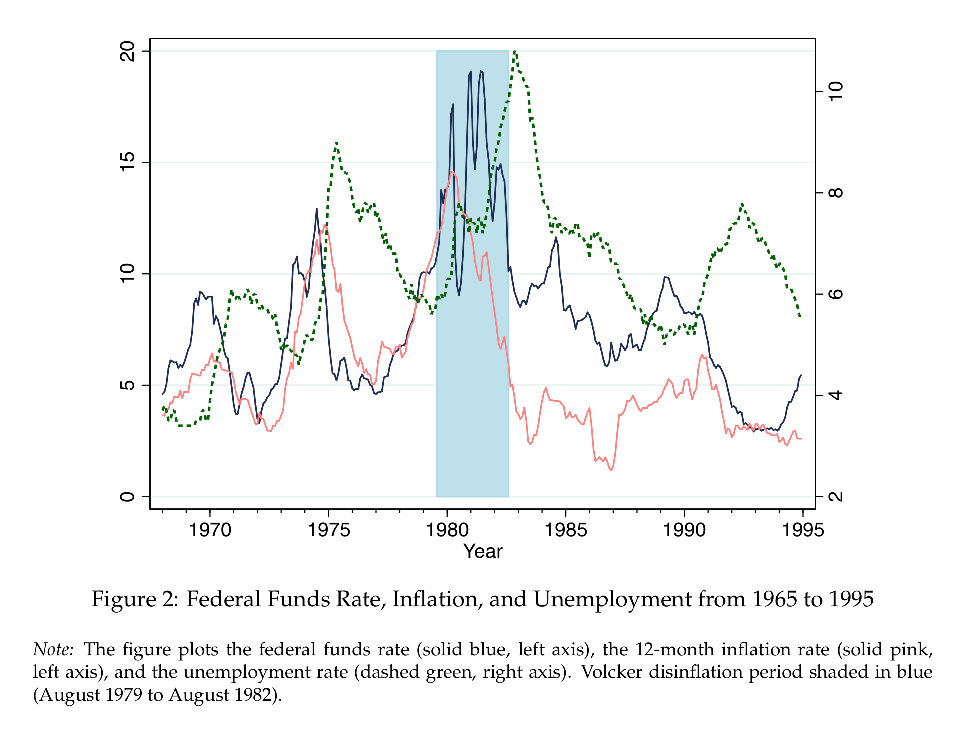
\includegraphics[scale=.6]{nakamura_steinsson.eps}
  \end{figure}
  Nakamura \& Steinsson (2017)
\end{frame}
%--------------------------------------

%--------------------------------------
\begin{frame}
  \begin{figure}
    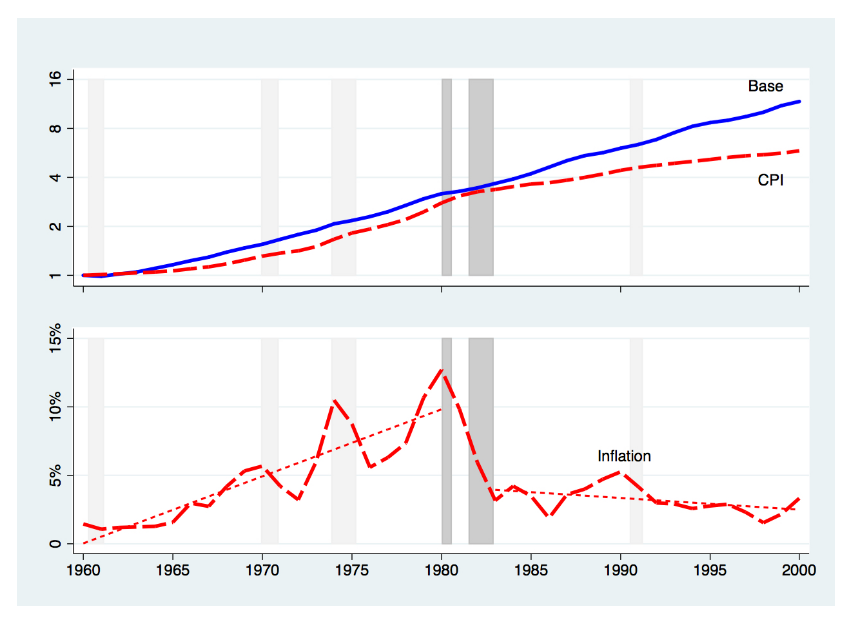
\includegraphics[scale=.7]{romer.eps}
  \end{figure}
  Romer (2016)
\end{frame}
%--------------------------------------

%--------------------------------------
\begin{frame}
  During the 1980s output seemed indeed to respond to monetary policy, but there are other factors
  \begin{enumerate}
    \item Oil shocks in 1979/1980
    \item Credit controls in 1980
    \item Tax cuts in 1981-82
  \end{enumerate}
  \medskip
  Volcker episode is consistent with non-neutrality of monetary policy, but not concerning idea that policy affects output with long and variable lags.
  \begin{itemize}
    \item Indeed output reacted largely synchronised with FED actions
  \end{itemize}  
\end{frame}
%--------------------------------------

%--------------------------------------
\begin{frame}
  Searching for natural experiments can also be done using the narrative record, which is what Romer \& Romer (1989) did.
  \begin{itemize}
    \item They use Federal Reserve records to identify natural experiments
    \item Looking at attempt to exert contractionary influence on the economy to reduce inflation
  \end{itemize}
  \medskip
  Their paper is based on the earlier mentioned work by Friedman \& Schwartz.
\end{frame}
%--------------------------------------

%--------------------------------------
\begin{frame}
  \begin{figure}
    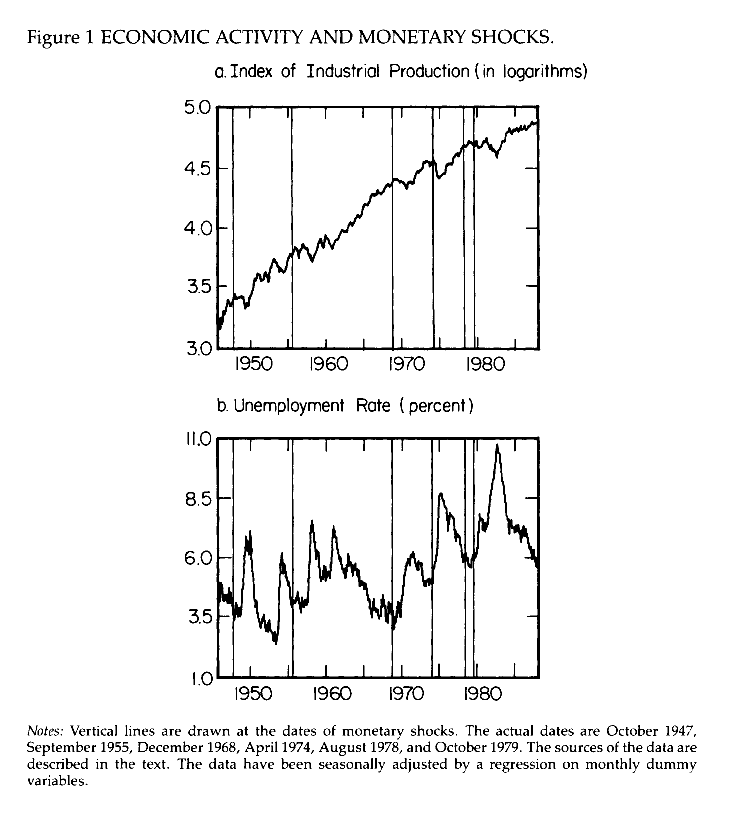
\includegraphics[scale=.6]{romer_romer.eps}
  \end{figure}
  Romer \& Romer (1989)
\end{frame}
%--------------------------------------

%--------------------------------------
\begin{frame}
  Although interesting, there are some shortcomings with this approach
  \begin{enumerate}
    \item Unclear how narrative record is selected; risk of reverse-engineering 
    \item Few data points; some other factor might be correlated with monetary shock, e.g. oil shocks
    \item Shock are endogenous because they might be predictable; hard to establish though
  \end{enumerate}
\end{frame}
%--------------------------------------

%--------------------------------------
\begin{frame}
  There is reduced-form evidence that monetary policy affects relative price based on discontinuity-based identification methods. 
  Seminal paper here is Mussa (1986) who used abrupt change in monetary policy following the breakdown of the Bretton Woods system of fixed exchange rate.
  \begin{itemize}
    \item Breakdown in  February 1973 caused large increase in volatility of US exchange rate        
  \end{itemize}  
\end{frame}
%--------------------------------------

%--------------------------------------
\begin{frame}
 Switching from a fixed to flexible exchange rate is a strictly monetary action. 
 \begin{itemize}
   \item If monetary policy has no real effects, this shouldn't have an impact on real variables such as the real exchange rate
 \end{itemize}
  \medskip
  NB - In discontinuity-based design the identifying assumption made is that other factors affecting the exchange rate do not change discontinuously.
\end{frame}
%--------------------------------------

%--------------------------------------
\begin{frame}
  \begin{figure}
    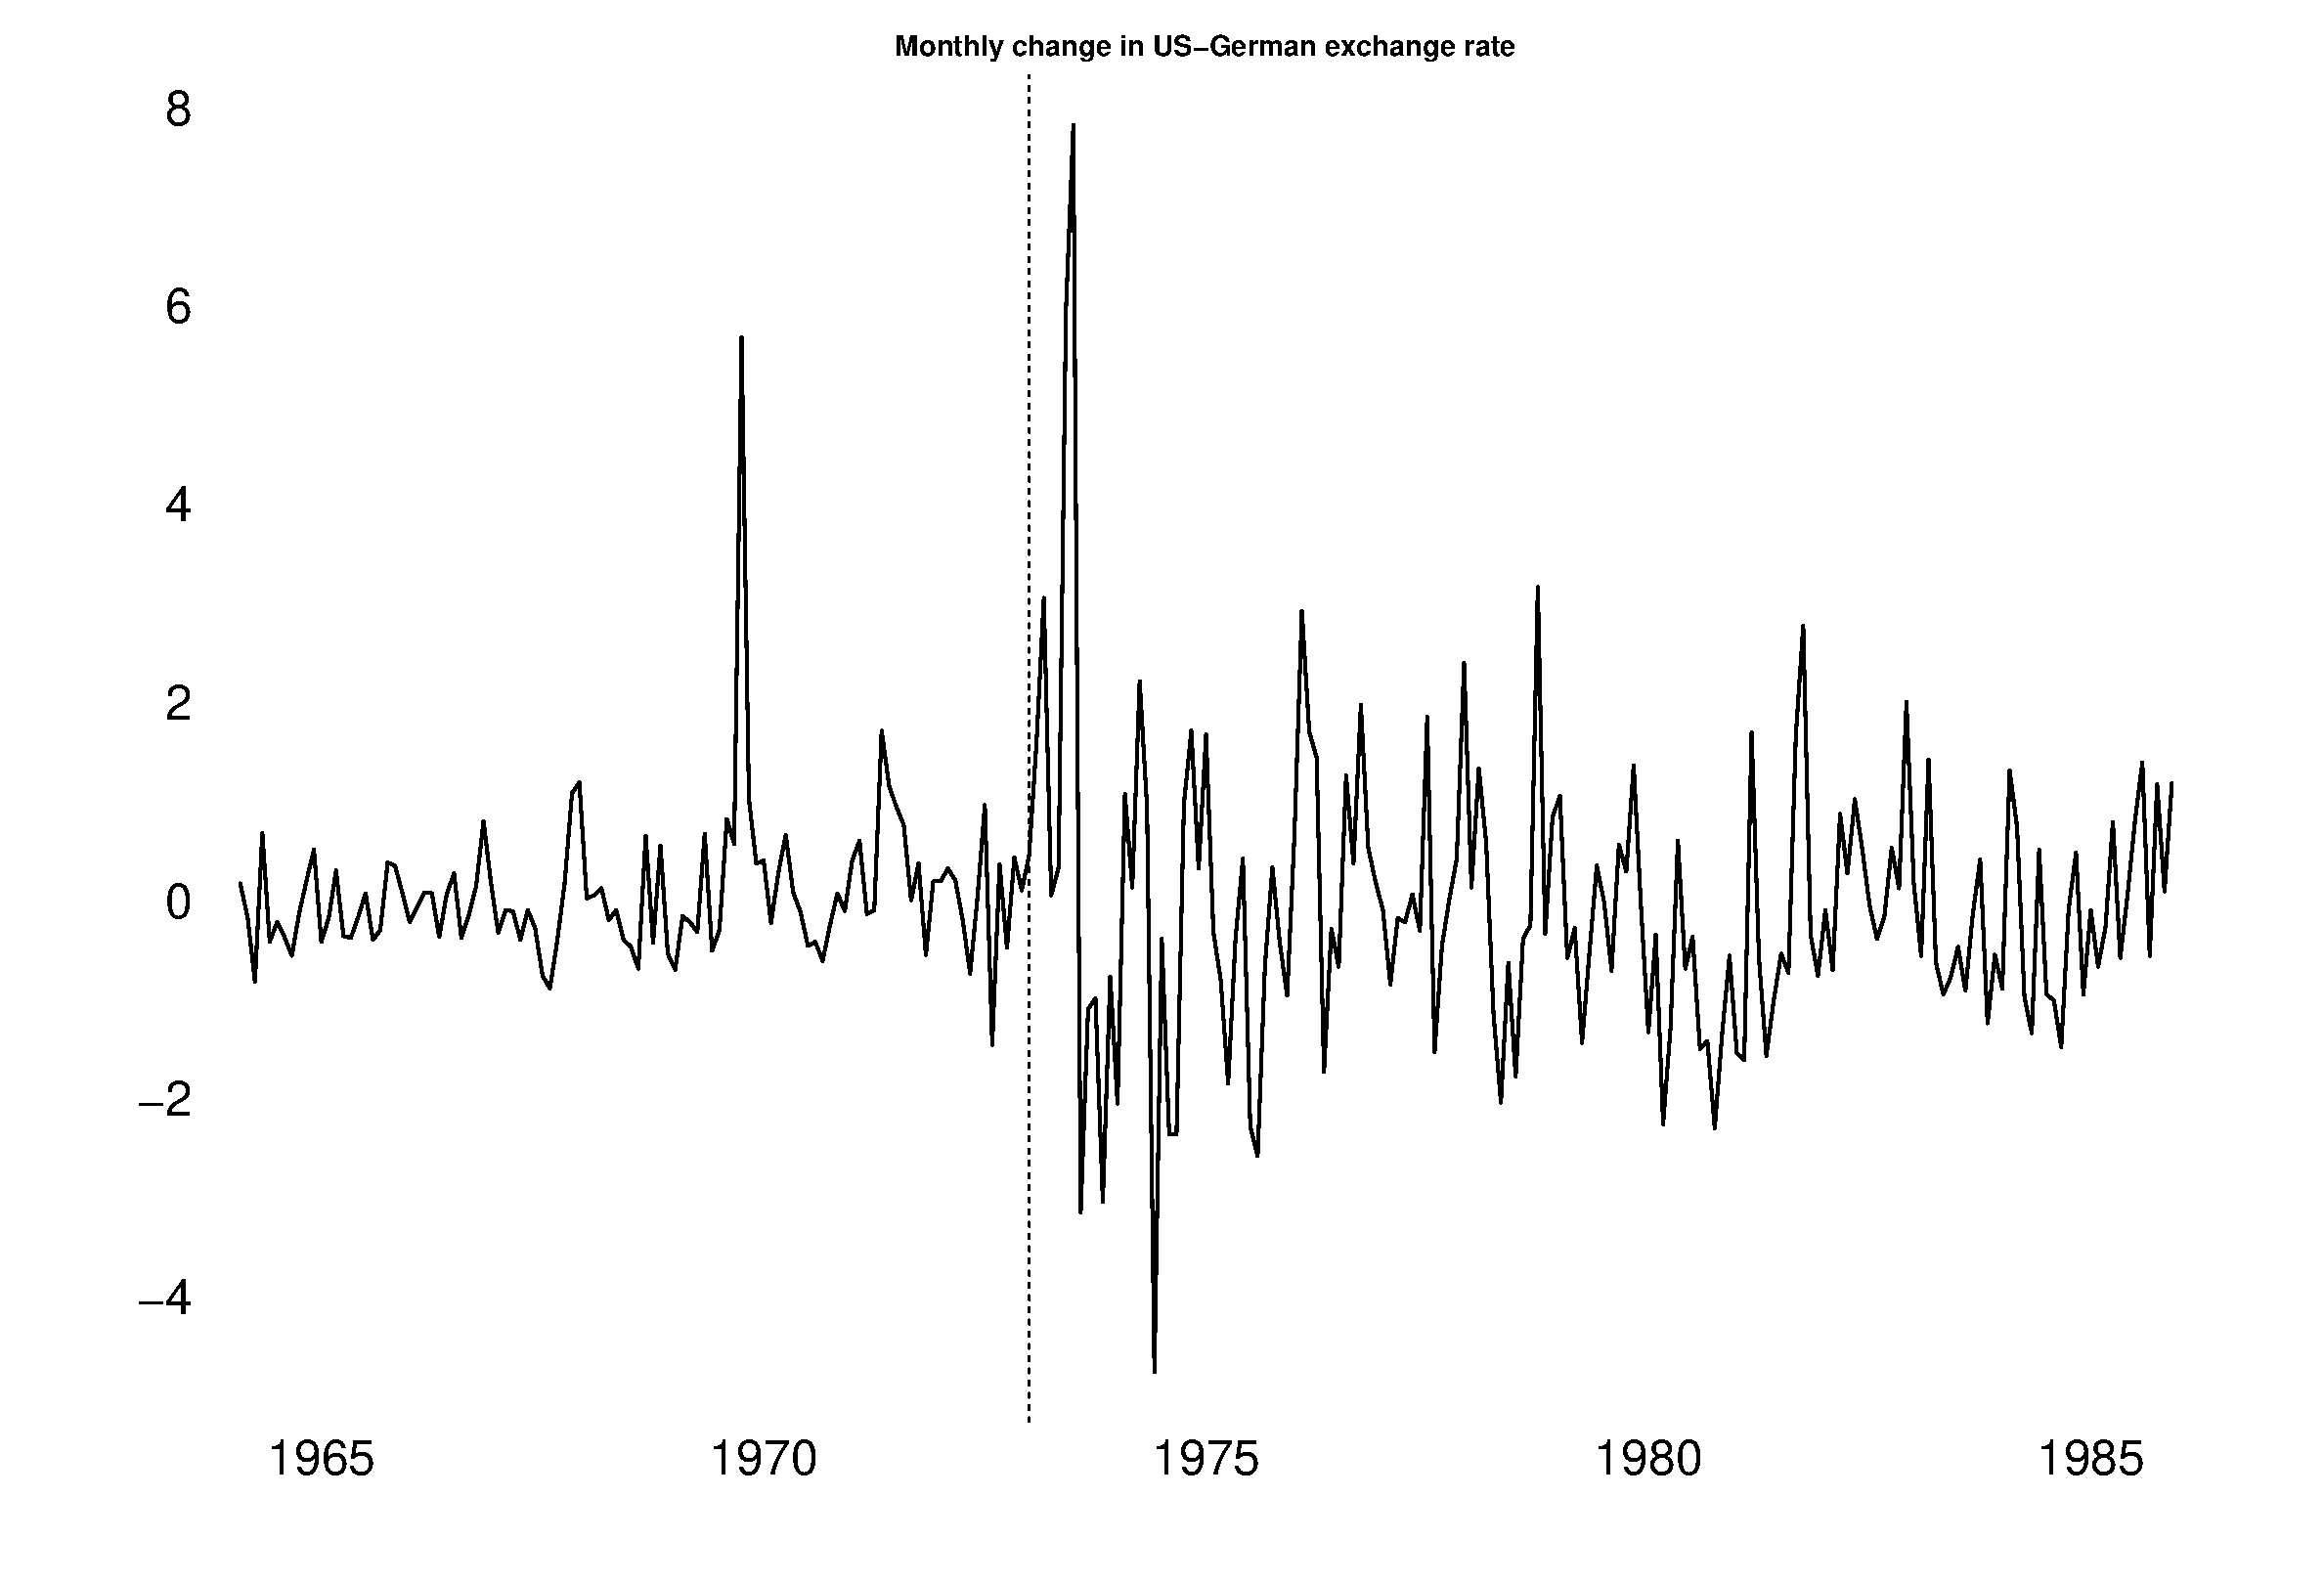
\includegraphics[scale=.3]{exchange_rate.eps}
  \end{figure}  
\end{frame}
%--------------------------------------

%--------------------------------------
\end{document}
